% questions.tex —— 1997 年·普通高等学校招生考试·全国卷文科 · 题目内容片段（无答案）
% 由 tools/generate_projects.py 依来源总账自 1997/1997_数学真题_全国文_试题.md 生成，勿手改（改源 MD 后重跑）


\gkpart{文科数学}

\begin{gktip}
\textbf{来源说明}：本题面按固定源 PDF 第 1 页（A3 横向、印刷页 55）逐题转录并完成独立逐题对照。固定来源的出版者、版次、复制链和官方身份未核；PDF 只含题面，不含答案、解析或评分标准。答案为本库独立推导，官方答案字段仍为空。

\textbf{未决原文缺字}：第 23 题（3）固定源在“面 AED”与“面 A1FD1”之间未印关系符号，正文以【原卷缺关系符号】占位。现有解析仅能给出“若符号为垂直则可证”的条件推论，不能据此判断原题关系；同版来源或可信勘误取得前保持未决。

\textbf{原文疑似排印错误}：第 25 题末句固定源印作“求该的圆的方程”，照录，不按语感修订。

\textbf{图形说明}：第 3 题四个函数图象选项及第 23 题正方体示意图依固定源图形关系重绘为 TikZ 矢量图。
\end{gktip}

\gkpart{选择题（第1—15题；分组为项目编辑结构）}

\begin{question}
\gkti{1}设集合 $M=\{x\mid0\le x<2\}$，集合 $N=\{x\mid x^2-2x-3<0\}$，集合 $M\cap N=$（　）。

（A）$\{x\mid0\le x<1\}$；（B）$\{x\mid0\le x<2\}$；（C）$\{x\mid0\le x\le1\}$；（D）$\{x\mid0\le x\le2\}$。

\end{question}
\begin{question}
\gkti{2}如果直线 $ax+2y+2=0$ 与直线 $3x-y-2=0$ 平行，那么系数 $a=$（　）。

（A）$-3$；（B）$-6$；（C）$-\dfrac32$；（D）$\dfrac23$。

\Needspace{0.4\textheight}
\end{question}
\begin{question}
\gkti{3}函数 $y=\tan\left(\dfrac12x-\dfrac\pi3\right)$ 在一个周期内的图象是（　）。

（A）图A；（B）图B；（C）图C；（D）图D。
\nopagebreak[4]
\begin{center}% 原页四个定性图的轴、零点、渐近线与标号；曲线形状按正切模型示意重建。
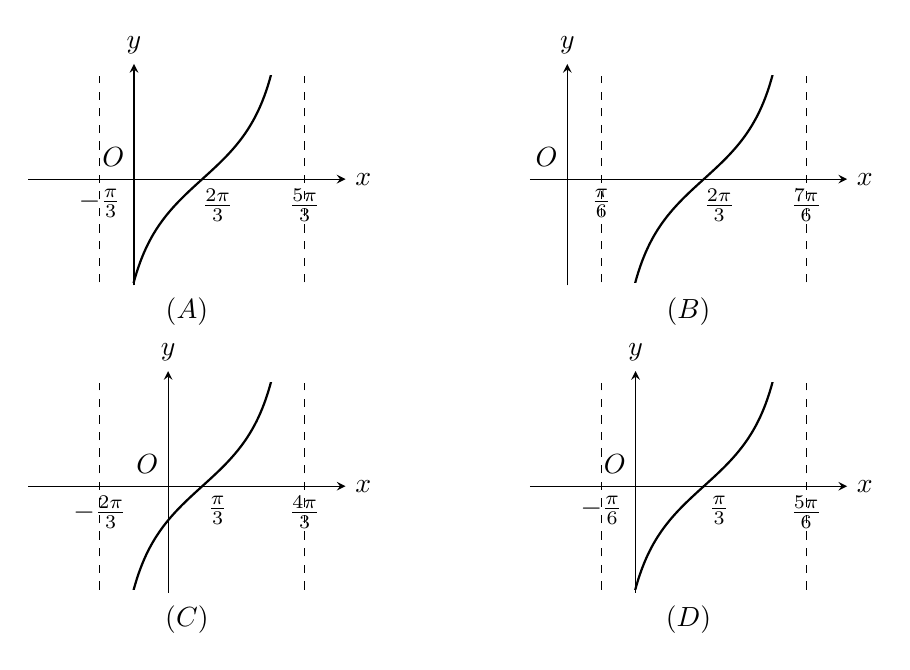
\begin{tikzpicture}[x=1.3cm,y=0.75cm,>=stealth]
\def\gkartsgraph#1#2#3#4#5{%
  \draw[->] (-1.7,0)--(1.4,0) node[right] {$x$};
  \draw[->] (#1,-1.8)--(#1,1.95) node[above] {$y$};
  \draw[dashed] (-1,-1.75)--(-1,1.75) (1,-1.75)--(1,1.75);
  \begin{scope}
    \clip (-1.7,-1.75) rectangle (1.4,1.75);
    \draw[thick,samples=100,domain=-0.92:0.92] plot (\x,{tan(90*\x)});
  \end{scope}
  \node[below] at (-1,0) {$#2$};
  \node[below] at (0.15,0) {$#3$};
  \node[below] at (1,0) {$#4$};
  \node[above left,yshift=1pt] at (#1,0) {$O$};
  \node at (-0.15,-2.25) {$(#5)$};
}
\begin{scope}
\gkartsgraph{-0.6667}{-\frac\pi3}{\frac{2\pi}3}{\frac{5\pi}3}{A}
\end{scope}
\begin{scope}[shift={(4.9,0)}]
\gkartsgraph{-1.3333}{\frac\pi6}{\frac{2\pi}3}{\frac{7\pi}6}{B}
\end{scope}
\begin{scope}[shift={(0,-5.2)}]
\gkartsgraph{-0.3333}{-\frac{2\pi}3}{\frac\pi3}{\frac{4\pi}3}{C}
\end{scope}
\begin{scope}[shift={(4.9,-5.2)}]
\gkartsgraph{-0.6667}{-\frac\pi6}{\frac\pi3}{\frac{5\pi}6}{D}
\end{scope}
\end{tikzpicture}
\end{center}
\nopagebreak[4]
\end{question}
\begin{question}
\gkti{4}已知三棱锥 $D-ABC$ 的三个侧面与底面全等，且 $AB=AC=\sqrt3$，$BC=2$，则以 $BC$ 为棱、以面 $BCD$ 与面 $BCA$ 为面的二面角的大小是（　）。

（A）$\dfrac\pi4$；（B）$\dfrac\pi3$；（C）$\dfrac\pi2$；（D）$\dfrac{2\pi}3$。

\end{question}
\begin{question}
\gkti{5}函数 $y=\sin\left(\dfrac\pi3-2x\right)+\sin2x$ 的最小正周期是（　）。

（A）$\dfrac\pi2$；（B）$\pi$；（C）$2\pi$；（D）$4\pi$。

\end{question}
\begin{question}
\gkti{6}满足 $\tan\alpha\ge\cot\alpha$ 的 $\alpha$ 的一个取值区间是（　）。

（A）$\left(0,\dfrac\pi4\right]$；（B）$\left[0,\dfrac\pi4\right]$；（C）$\left[\dfrac\pi4,\dfrac\pi2\right)$；（D）$\left[\dfrac\pi4,\dfrac\pi2\right]$。

\end{question}
\begin{question}
\gkti{7}设函数 $y=f(x)$ 定义在实数集上，则函数 $y=f(x-1)$ 与 $y=f(1-x)$ 的图象关于（　）。

（A）直线 $y=0$ 对称；（B）直线 $x=0$ 对称；（C）直线 $y=1$ 对称；（D）直线 $x=1$ 对称。

\end{question}
\begin{question}
\gkti{8}长方体一个顶点上三条棱的长分别是 $3,4,5$，且它的八个顶点都在同一个球面上，这个球的表面积是（　）。

（A）$20\sqrt2\pi$；（B）$25\sqrt2\pi$；（C）$50\pi$；（D）$200\pi$。

\end{question}
\begin{question}
\gkti{9}如果直线 $l$ 将圆 $x^2+y^2-2x-4y=0$ 平分，且不通过第四象限，那么 $l$ 的斜率的取值范围是（　）。

（A）$[0,2]$；（B）$[0,1]$；（C）$\left[0,\dfrac12\right]$；（D）$\left[0,\dfrac12\right)$。

\end{question}
\begin{question}
\gkti{10}函数 $y=\cos^2x-3\cos x+2$ 的最小值为（　）。

（A）$2$；（B）$0$；（C）$-\dfrac14$；（D）$6$。

\end{question}
\begin{question}
\gkti{11}椭圆 $C$ 与椭圆 $\dfrac{(x-3)^2}{9}+\dfrac{(y-2)^2}{4}=1$ 关于直线 $x+y=0$ 对称，椭圆 $C$ 的方程是（　）。

（A）$\dfrac{(x+2)^2}{4}+\dfrac{(y+3)^2}{9}=1$；（B）$\dfrac{(x-2)^2}{9}+\dfrac{(y-3)^2}{4}=1$；

（C）$\dfrac{(x+2)^2}{9}+\dfrac{(y+3)^2}{4}=1$；（D）$\dfrac{(x-2)^2}{4}+\dfrac{(y-3)^2}{9}=1$。

\end{question}
\begin{question}
\gkti{12}圆台上、下底面积分别为 $\pi,4\pi$，侧面积为 $6\pi$，这个圆台的体积是（　）。

（A）$\dfrac{2\sqrt3\pi}{3}$；（B）$2\sqrt3\pi$；（C）$\dfrac{7\sqrt3\pi}{6}$；（D）$\dfrac{7\sqrt3\pi}{3}$。

\end{question}
\begin{question}
\gkti{13}定义在区间 $(-\infty,+\infty)$ 的奇函数 $f(x)$ 为增函数，偶函数 $g(x)$ 在区间 $[0,+\infty)$ 的图象与 $f(x)$ 的图象重合，设 $a>b>0$，给出下列不等式：

① $f(b)-f(-a)>g(a)-g(-b)$；② $f(b)-f(-a)<g(a)-g(-b)$；

③ $f(a)-f(-b)>g(b)-g(-a)$；④ $f(a)-f(-b)<g(b)-g(-a)$。

其中成立的是（　）。

（A）①与④；（B）②与③；（C）①与③；（D）②与④。

\end{question}
\begin{question}
\gkti{14}不等式组

\nopagebreak[4]
\[
\begin{cases}
x>0,\\
\dfrac{3-x}{3+x}>\left|\dfrac{2-x}{2+x}\right|
\end{cases}
\]

的解集是（　）。

（A）$\{x\mid0<x<2\}$；（B）$\{x\mid0<x<2.5\}$；（C）$\{x\mid0<x<\sqrt6\}$；（D）$\{x\mid0<x<3\}$。

\end{question}
\begin{question}
\gkti{15}四面体的一个顶点为 $A$，从其他顶点与棱的中点中取 $3$ 个点，使它们和点 $A$ 在同一平面上，不同的取法共有（　）。

（A）30种；（B）33种；（C）36种；（D）39种。

\end{question}
\gkpart{填空题（第16—19题；分组为项目编辑结构）}

\begin{question}
\gkti{16}已知 $\left(\dfrac ax-\sqrt{\dfrac x2}\right)^9$ 的展开式中 $x^3$ 的系数为 $\dfrac94$，常数 $a$ 的值为\gkblank{}。

\end{question}
\begin{question}
\gkti{17}已知直线 $x-y=2$ 与抛物线 $y^2=4x$ 交于 $A,B$ 两点，那么线段 $AB$ 的中点坐标是\gkblank{}。

\end{question}
\begin{question}
\gkti{18}$\dfrac{\sin7^\circ+\cos15^\circ\sin8^\circ}{\cos7^\circ-\sin15^\circ\sin8^\circ}$ 的值为\gkblank{}。

\end{question}
\begin{question}
\gkti{19}已知 $m,l$ 是直线，$\alpha,\beta$ 是平面，给出下列命题：

① 若 $l$ 垂直于 $\alpha$ 内的两条相交直线，则 $l\perp\alpha$；

② 若 $l$ 平行于 $\alpha$，则 $l$ 平行于 $\alpha$ 内的所有直线；

③ 若 $m\subset\alpha$，$l\subset\beta$，且 $l\perp m$，则 $\alpha\perp\beta$；

④ 若 $l\subset\beta$，且 $l\perp\alpha$，则 $\alpha\perp\beta$；

⑤ 若 $m\subset\alpha$，$l\subset\beta$，且 $\alpha\parallel\beta$，则 $m\parallel l$。

其中正确的命题的序号是\gkblank{}。（注：把你认为正确的命题的序号都填上）

\end{question}
\gkpart{解答题（第20—25题；分组为项目编辑结构）}

\begin{question}
\gkti{20}已知复数 $z=\dfrac12+\dfrac{\sqrt3}{2}i$，$\omega=\dfrac{\sqrt2}{2}+\dfrac{\sqrt2}{2}i$。求复数 $z\omega+z\omega^3$ 的模及辐角主值。

\end{question}
\begin{question}
\gkti{21}设 $S_n$ 是等差数列 $\{a_n\}$ 前 $n$ 项的和。已知 $\dfrac{S_3}{3}$ 与 $\dfrac{S_4}{4}$ 的等比中项为 $\dfrac{S_1}{5}$，$\dfrac{S_3}{3}$ 与 $\dfrac{S_4}{4}$ 的等差中项为 $1$。求等差数列 $\{a_n\}$ 的通项 $a_n$。

\end{question}
\begin{question}
\gkti{22}甲、乙两地相距 $S$ 千米，汽车从甲地匀速行驶到乙地，速度不得超过 $c$ 千米/时。已知汽车每小时的运输成本（以元为单位）由可变部分和固定部分组成：可变部分与速度 $v$（千米/时）的平方成正比，比例系数为 $b$；固定部分为 $a$ 元。

（1） 把全程运输成本 $y$（元）表示为速度 $v$（千米/时）的函数，并指出这个函数的定义域；

（2） 为了使全程运输成本最小，汽车应以多大速度行驶？

\Needspace{0.4\textheight}
\end{question}
\begin{question}
\gkti{23}如图，在正方体 $ABCD-A_1B_1C_1D_1$ 中，$E,F$ 分别是 $BB_1,CD$ 的中点。

（1） 证明：$AD\perp D_1F$；

（2） 求 $AE$ 与 $D_1F$ 所成的角；

（3） 证明：面 $AED$【原卷缺关系符号】面 $A_1FD_1$；

\begin{gktip}
来源缺口：上行两平面之间未印关系符号。此处保留可见文字，不自行补成垂直、平行或其他关系；该小问待补源。
\end{gktip}

（4） 设 $AA_1=2$，求三棱锥 $F-A_1ED_1$ 的体积。
\nopagebreak[4]
\begin{center}% 依固定题面中正方体的点线关系重绘；投影不表示长度、角度比例。
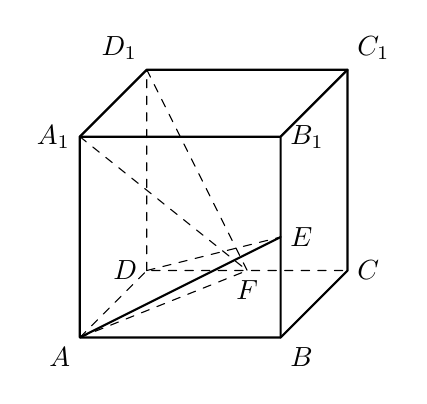
\begin{tikzpicture}[scale=0.85,line join=round,line cap=round]
\coordinate (A) at (0,0);
\coordinate (B) at (3,0);
\coordinate (C) at (4,1);
\coordinate (D) at (1,1);
\coordinate (Aone) at (0,3);
\coordinate (Bone) at (3,3);
\coordinate (Cone) at (4,4);
\coordinate (Done) at (1,4);
\coordinate (E) at (3,1.5);
\coordinate (F) at (2.5,1);
\draw[thick] (A)--(B)--(C)--(Cone)--(Done)--(Aone)--cycle;
\draw[thick] (Aone)--(Bone)--(Cone) (B)--(Bone);
\draw[dashed] (A)--(D)--(C) (D)--(Done);
\draw[thick] (A)--(E);
\draw[dashed] (D)--(E) (A)--(F) (Aone)--(F) (Done)--(F);
\node[below left] at (A) {$A$};
\node[below right] at (B) {$B$};
\node[right] at (C) {$C$};
\node[left] at (D) {$D$};
\node[left] at (Aone) {$A_1$};
\node[right] at (Bone) {$B_1$};
\node[above right] at (Cone) {$C_1$};
\node[above left] at (Done) {$D_1$};
\node[right] at (E) {$E$};
\node[below] at (F) {$F$};
\end{tikzpicture}
\end{center}
\nopagebreak[4]
\end{question}
\begin{question}
\gkti{24}已知过原点 $O$ 的一条直线与函数 $y=\log_8x$ 的图象交于 $A,B$ 两点，分别过点 $A,B$ 作 $y$ 轴的平行线与函数的 $y=\log_2x$ 的图象交于 $C,D$ 两点。

（1） 证明：点 $C,D$ 和原点 $O$ 在同一条直线上；

（2） 当 $BC$ 平行于 $x$ 轴时，求点 $A$ 的坐标。

\end{question}
\begin{question}
\gkti{25}设圆满足：① 截 $y$ 轴所得弦长为 $2$；② 被 $x$ 轴分成两段圆弧，其弧长的比为 $3:1$；③ 圆心到直线 $l:x-2y=0$ 的距离为 $\dfrac{\sqrt5}{5}$。求该的圆的方程。

\end{question}